\documentclass[1p]{elsarticle_modified}
%\bibliographystyle{elsarticle-num}

%\usepackage[colorlinks]{hyperref}
%\usepackage{abbrmath_seonhwa} %\Abb, \Ascr, \Acal ,\Abf, \Afrak
\usepackage{amsfonts}
\usepackage{amssymb}
\usepackage{amsmath}
\usepackage{amsthm}
\usepackage{scalefnt}
\usepackage{amsbsy}
\usepackage{kotex}
\usepackage{caption}
\usepackage{subfig}
\usepackage{color}
\usepackage{graphicx}
\usepackage{xcolor} %% white, black, red, green, blue, cyan, magenta, yellow
\usepackage{float}
\usepackage{setspace}
\usepackage{hyperref}

\usepackage{tikz}
\usetikzlibrary{arrows}

\usepackage{multirow}
\usepackage{array} % fixed length table
\usepackage{hhline}

%%%%%%%%%%%%%%%%%%%%%
\makeatletter
\renewcommand*\env@matrix[1][\arraystretch]{%
	\edef\arraystretch{#1}%
	\hskip -\arraycolsep
	\let\@ifnextchar\new@ifnextchar
	\array{*\c@MaxMatrixCols c}}
\makeatother %https://tex.stackexchange.com/questions/14071/how-can-i-increase-the-line-spacing-in-a-matrix
%%%%%%%%%%%%%%%

\usepackage[normalem]{ulem}

\newcommand{\msout}[1]{\ifmmode\text{\sout{\ensuremath{#1}}}\else\sout{#1}\fi}
%SOURCE: \msout is \stkout macro in https://tex.stackexchange.com/questions/20609/strikeout-in-math-mode

\newcommand{\cancel}[1]{
	\ifmmode
	{\color{red}\msout{#1}}
	\else
	{\color{red}\sout{#1}}
	\fi
}

\newcommand{\add}[1]{
	{\color{blue}\uwave{#1}}
}

\newcommand{\replace}[2]{
	\ifmmode
	{\color{red}\msout{#1}}{\color{blue}\uwave{#2}}
	\else
	{\color{red}\sout{#1}}{\color{blue}\uwave{#2}}
	\fi
}

\newcommand{\Sol}{\mathcal{S}} %segment
\newcommand{\D}{D} %diagram
\newcommand{\A}{\mathcal{A}} %arc


%%%%%%%%%%%%%%%%%%%%%%%%%%%%%5 test

\def\sl{\operatorname{\textup{SL}}(2,\Cbb)}
\def\psl{\operatorname{\textup{PSL}}(2,\Cbb)}
\def\quan{\mkern 1mu \triangleright \mkern 1mu}

\theoremstyle{definition}
\newtheorem{thm}{Theorem}[section]
\newtheorem{prop}[thm]{Proposition}
\newtheorem{lem}[thm]{Lemma}
\newtheorem{ques}[thm]{Question}
\newtheorem{cor}[thm]{Corollary}
\newtheorem{defn}[thm]{Definition}
\newtheorem{exam}[thm]{Example}
\newtheorem{rmk}[thm]{Remark}
\newtheorem{alg}[thm]{Algorithm}

\newcommand{\I}{\sqrt{-1}}
\begin{document}

%\begin{frontmatter}
%
%\title{Boundary parabolic representations of knots up to 8 crossings}
%
%%% Group authors per affiliation:
%\author{Yunhi Cho} 
%\address{Department of Mathematics, University of Seoul, Seoul, Korea}
%\ead{yhcho@uos.ac.kr}
%
%
%\author{Seonhwa Kim} %\fnref{s_kim}}
%\address{Center for Geometry and Physics, Institute for Basic Science, Pohang, 37673, Korea}
%\ead{ryeona17@ibs.re.kr}
%
%\author{Hyuk Kim}
%\address{Department of Mathematical Sciences, Seoul National University, Seoul 08826, Korea}
%\ead{hyukkim@snu.ac.kr}
%
%\author{Seokbeom Yoon}
%\address{Department of Mathematical Sciences, Seoul National University, Seoul, 08826,  Korea}
%\ead{sbyoon15@snu.ac.kr}
%
%\begin{abstract}
%We find all boundary parabolic representation of knots up to 8 crossings.
%
%\end{abstract}
%\begin{keyword}
%    \MSC[2010] 57M25 
%\end{keyword}
%
%\end{frontmatter}

%\linenumbers
%\tableofcontents
%
\newcommand\colored[1]{\textcolor{white}{\rule[-0.35ex]{0.8em}{1.4ex}}\kern-0.8em\color{red} #1}%
%\newcommand\colored[1]{\textcolor{white}{ #1}\kern-2.17ex	\textcolor{white}{ #1}\kern-1.81ex	\textcolor{white}{ #1}\kern-2.15ex\color{red}#1	}

{\Large $\underline{12a_{1182}~(K12a_{1182})}$}

\setlength{\tabcolsep}{10pt}
\renewcommand{\arraystretch}{1.6}
\vspace{1cm}\begin{tabular}{m{100pt}>{\centering\arraybackslash}m{274pt}}
\multirow{5}{120pt}{
	\centering
	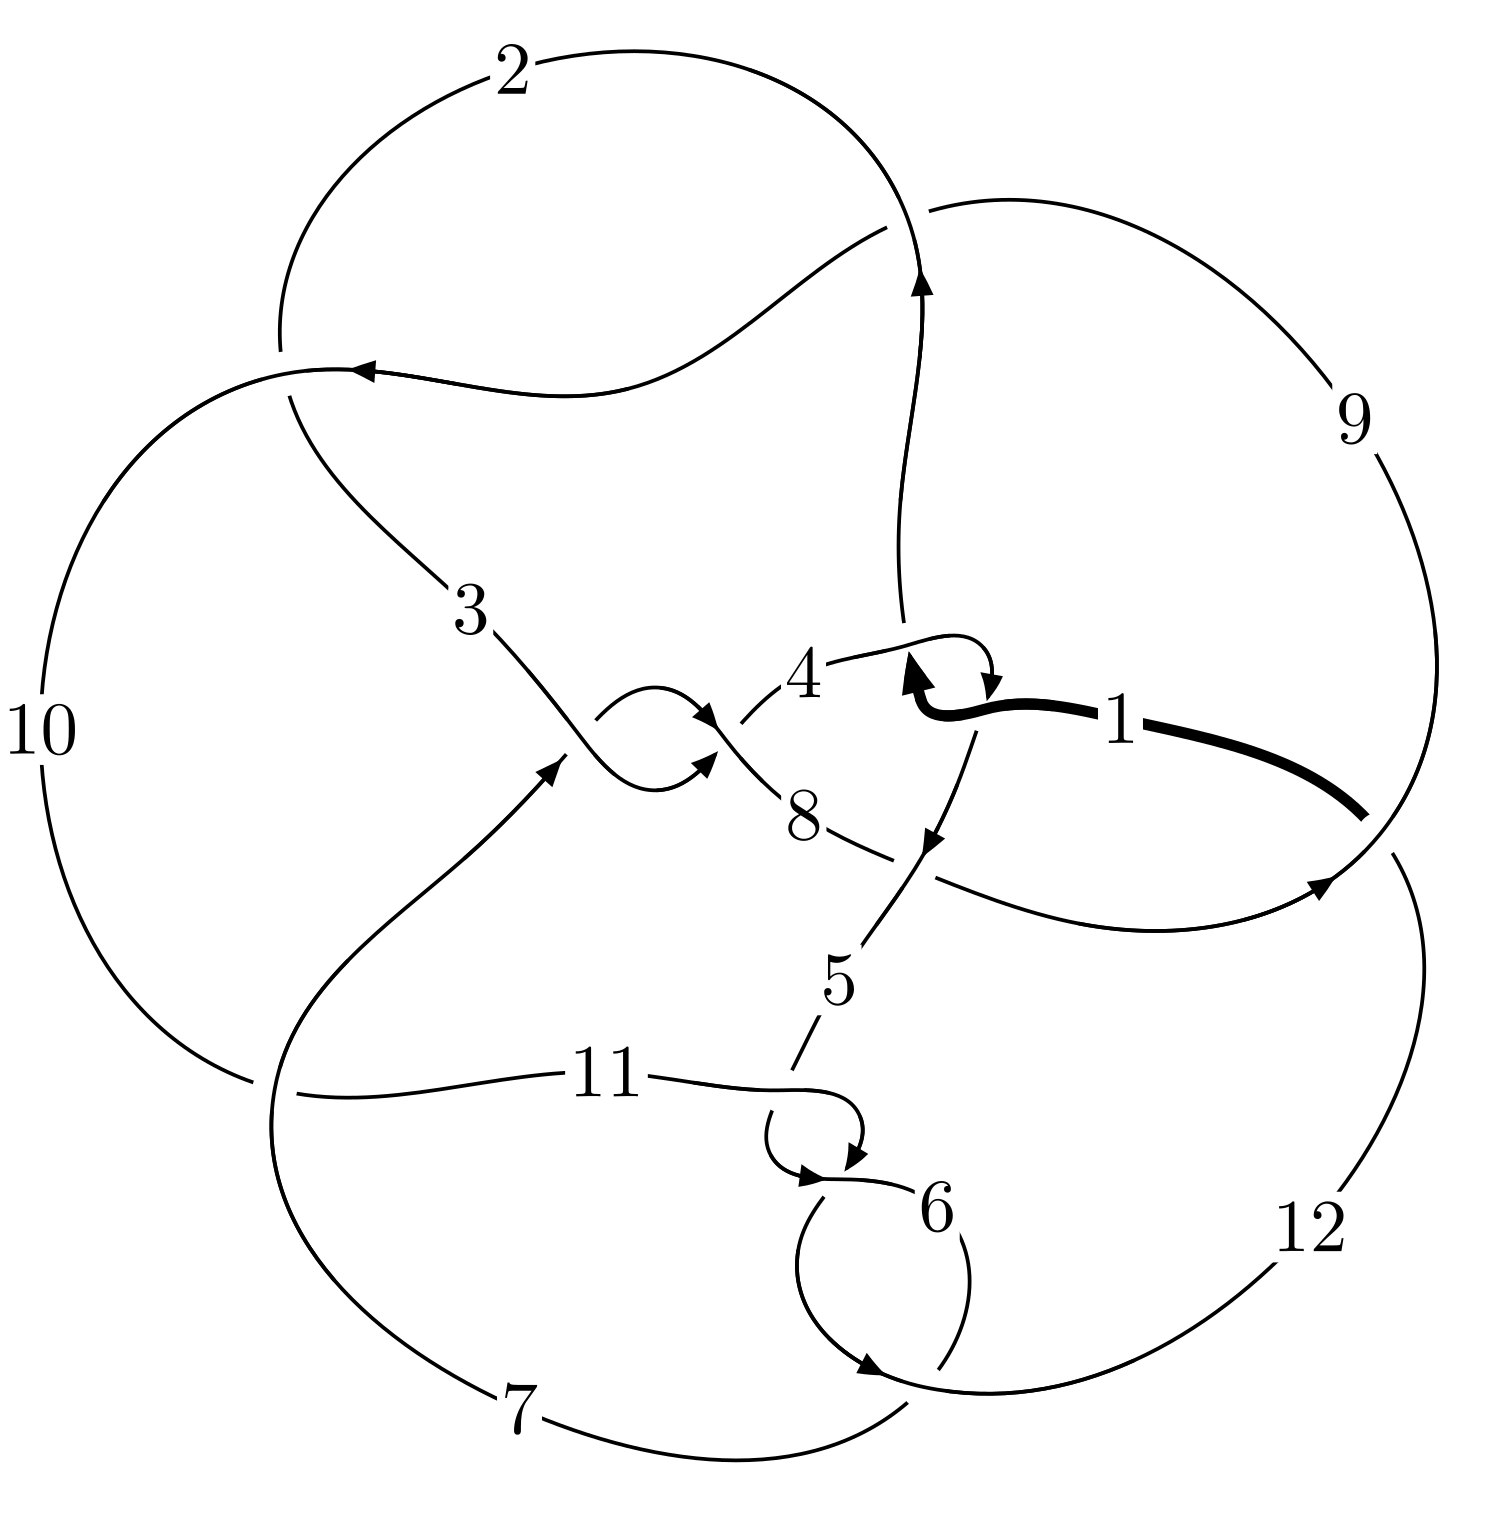
\includegraphics[width=112pt]{../../../GIT/diagram.site/Diagrams/png/1983_12a_1182.png}\\
\ \ \ A knot diagram\footnotemark}&
\allowdisplaybreaks
\textbf{Linearized knot diagam} \\
\cline{2-2}
 &
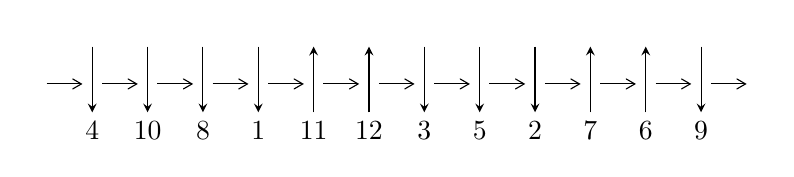
\begin{tikzpicture}[x=20pt, y=17pt]
	% nodes
	\node (C0) at (0, 0) {};
	\node (C1) at (1, 0) {};
	\node (C1U) at (1, +1) {};
	\node (C1D) at (1, -1) {4};

	\node (C2) at (2, 0) {};
	\node (C2U) at (2, +1) {};
	\node (C2D) at (2, -1) {10};

	\node (C3) at (3, 0) {};
	\node (C3U) at (3, +1) {};
	\node (C3D) at (3, -1) {8};

	\node (C4) at (4, 0) {};
	\node (C4U) at (4, +1) {};
	\node (C4D) at (4, -1) {1};

	\node (C5) at (5, 0) {};
	\node (C5U) at (5, +1) {};
	\node (C5D) at (5, -1) {11};

	\node (C6) at (6, 0) {};
	\node (C6U) at (6, +1) {};
	\node (C6D) at (6, -1) {12};

	\node (C7) at (7, 0) {};
	\node (C7U) at (7, +1) {};
	\node (C7D) at (7, -1) {3};

	\node (C8) at (8, 0) {};
	\node (C8U) at (8, +1) {};
	\node (C8D) at (8, -1) {5};

	\node (C9) at (9, 0) {};
	\node (C9U) at (9, +1) {};
	\node (C9D) at (9, -1) {2};

	\node (C10) at (10, 0) {};
	\node (C10U) at (10, +1) {};
	\node (C10D) at (10, -1) {7};

	\node (C11) at (11, 0) {};
	\node (C11U) at (11, +1) {};
	\node (C11D) at (11, -1) {6};

	\node (C12) at (12, 0) {};
	\node (C12U) at (12, +1) {};
	\node (C12D) at (12, -1) {9};
	\node (C13) at (13, 0) {};

	% arrows
	\draw[->,>={angle 60}]
	(C0) edge (C1) (C1) edge (C2) (C2) edge (C3) (C3) edge (C4) (C4) edge (C5) (C5) edge (C6) (C6) edge (C7) (C7) edge (C8) (C8) edge (C9) (C9) edge (C10) (C10) edge (C11) (C11) edge (C12) (C12) edge (C13) ;	\draw[->,>=stealth]
	(C1U) edge (C1D) (C2U) edge (C2D) (C3U) edge (C3D) (C4U) edge (C4D) (C5D) edge (C5U) (C6D) edge (C6U) (C7U) edge (C7D) (C8U) edge (C8D) (C9U) edge (C9D) (C10D) edge (C10U) (C11D) edge (C11U) (C12U) edge (C12D) ;
	\end{tikzpicture} \\
\hhline{~~} \\& 
\textbf{Solving Sequence} \\ \cline{2-2} 
 &
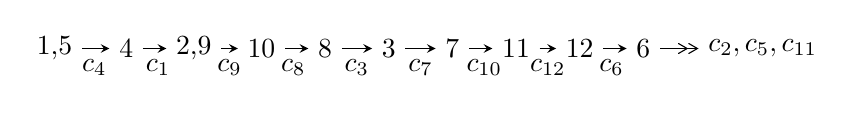
\begin{tikzpicture}[x=23pt, y=7pt]
	% node
	\node (A0) at (-1/8, 0) {1,5};
	\node (A1) at (1, 0) {4};
	\node (A2) at (33/16, 0) {2,9};
	\node (A3) at (25/8, 0) {10};
	\node (A4) at (33/8, 0) {8};
	\node (A5) at (41/8, 0) {3};
	\node (A6) at (49/8, 0) {7};
	\node (A7) at (57/8, 0) {11};
	\node (A8) at (65/8, 0) {12};
	\node (A9) at (73/8, 0) {6};
	\node (C1) at (1/2, -1) {$c_{4}$};
	\node (C2) at (3/2, -1) {$c_{1}$};
	\node (C3) at (21/8, -1) {$c_{9}$};
	\node (C4) at (29/8, -1) {$c_{8}$};
	\node (C5) at (37/8, -1) {$c_{3}$};
	\node (C6) at (45/8, -1) {$c_{7}$};
	\node (C7) at (53/8, -1) {$c_{10}$};
	\node (C8) at (61/8, -1) {$c_{12}$};
	\node (C9) at (69/8, -1) {$c_{6}$};
	\node (A10) at (11, 0) {$c_{2},c_{5},c_{11}$};

	% edge
	\draw[->,>=stealth]	
	(A0) edge (A1) (A1) edge (A2) (A2) edge (A3) (A3) edge (A4) (A4) edge (A5) (A5) edge (A6) (A6) edge (A7) (A7) edge (A8) (A8) edge (A9) ;
	\draw[->>,>={angle 60}]	
	(A9) edge (A10);
\end{tikzpicture} \\ 

\end{tabular} \\

\footnotetext{
The image of knot diagram is generated by the software ``\textbf{Draw programme}" developed by Andrew Bartholomew(\url{http://www.layer8.co.uk/maths/draw/index.htm\#Running-draw}), where we modified some parts for our purpose(\url{https://github.com/CATsTAILs/LinksPainter}).
}\phantom \\ \newline 
\centering \textbf{Ideals for irreducible components\footnotemark of $X_{\text{par}}$} 
 
\begin{align*}
I^u_{1}&=\langle 
-1393 u^{37}+27813 u^{36}+\cdots+128 b+48128,\;188 u^{37}-2555 u^{36}+\cdots+128 a+149824,\\
\phantom{I^u_{1}}&\phantom{= \langle  }u^{38}-21 u^{37}+\cdots-4864 u+256\rangle \\
I^u_{2}&=\langle 
-3.88208\times10^{52} a^{15} u^{4}+1.90625\times10^{52} a^{14} u^{4}+\cdots+3.57811\times10^{52} a+3.35225\times10^{51},\\
\phantom{I^u_{2}}&\phantom{= \langle  }- a^{15} u^4-6 a^{14} u^4+\cdots-102 a-31,\;u^5+u^4+2 u^3+u^2+u+1\rangle \\
I^u_{3}&=\langle 
-9 u^{24}-37 u^{23}+\cdots+b+37,\;-37 u^{24}-231 u^{23}+\cdots+a-6,\;u^{25}+6 u^{24}+\cdots+5 u+1\rangle \\
\\
\end{align*}
\raggedright * 3 irreducible components of $\dim_{\mathbb{C}}=0$, with total 143 representations.\\
\footnotetext{All coefficients of polynomials are rational numbers. But the coefficients are sometimes approximated in decimal forms when there is not enough margin.}
\newpage
\renewcommand{\arraystretch}{1}
\centering \section*{I. $I^u_{1}= \langle -1393 u^{37}+27813 u^{36}+\cdots+128 b+48128,\;188 u^{37}-2555 u^{36}+\cdots+128 a+149824,\;u^{38}-21 u^{37}+\cdots-4864 u+256 \rangle$}
\flushleft \textbf{(i) Arc colorings}\\
\begin{tabular}{m{7pt} m{180pt} m{7pt} m{180pt} }
\flushright $a_{1}=$&$\begin{pmatrix}0\\u\end{pmatrix}$ \\
\flushright $a_{5}=$&$\begin{pmatrix}1\\0\end{pmatrix}$ \\
\flushright $a_{4}=$&$\begin{pmatrix}1\\- u^2\end{pmatrix}$ \\
\flushright $a_{2}=$&$\begin{pmatrix}- u\\u^3+u\end{pmatrix}$ \\
\flushright $a_{9}=$&$\begin{pmatrix}-1.46875 u^{37}+19.9609 u^{36}+\cdots+21583.3 u-1170.50\\10.8828 u^{37}-217.289 u^{36}+\cdots+8314.50 u-376\end{pmatrix}$ \\
\flushright $a_{10}=$&$\begin{pmatrix}-15.7188 u^{37}+312.086 u^{36}+\cdots-11376.8 u+539.500\\6.07031 u^{37}-147.727 u^{36}+\cdots+72282.5 u-3910\end{pmatrix}$ \\
\flushright $a_{8}=$&$\begin{pmatrix}9.41406 u^{37}-197.328 u^{36}+\cdots+29897.8 u-1546.50\\10.8828 u^{37}-217.289 u^{36}+\cdots+8314.50 u-376\end{pmatrix}$ \\
\flushright $a_{3}=$&$\begin{pmatrix}-\frac{3}{256} u^{37}+\frac{77}{256} u^{36}+\cdots-159 u+9\\\frac{59}{128} u^{37}-\frac{1173}{128} u^{36}+\cdots+2170 u-121\end{pmatrix}$ \\
\flushright $a_{7}=$&$\begin{pmatrix}-13.9961 u^{37}+294.926 u^{36}+\cdots-43159.8 u+2266\\-8.22656 u^{37}+153.602 u^{36}+\cdots+27840 u-1591\end{pmatrix}$ \\
\flushright $a_{11}=$&$\begin{pmatrix}5.77734 u^{37}-105.535 u^{36}+\cdots-21165.3 u+1168.50\\-6.44531 u^{37}+137.477 u^{36}+\cdots-21511.5 u+1137\end{pmatrix}$ \\
\flushright $a_{12}=$&$\begin{pmatrix}-1.52734 u^{37}+31.5352 u^{36}+\cdots-7145 u+382\\\frac{69}{128} u^{37}-\frac{1515}{128} u^{36}+\cdots+7048 u-391\end{pmatrix}$ \\
\flushright $a_{6}=$&$\begin{pmatrix}-4.78906 u^{37}+89.7813 u^{36}+\cdots+14346.5 u-796\\\frac{185}{128} u^{37}-\frac{4709}{128} u^{36}+\cdots+16332 u-884\end{pmatrix}$\\&\end{tabular}
\flushleft \textbf{(ii) Obstruction class $= -1$}\\~\\
\flushleft \textbf{(iii) Cusp Shapes $= -\frac{129}{32} u^{37}+\frac{3399}{32} u^{36}+\cdots-67794 u+3762$}\\~\\
\newpage\renewcommand{\arraystretch}{1}
\flushleft \textbf{(iv) u-Polynomials at the component}\newline \\
\begin{tabular}{m{50pt}|m{274pt}}
Crossings & \hspace{64pt}u-Polynomials at each crossing \\
\hline $$\begin{aligned}c_{1},c_{4}\end{aligned}$$&$\begin{aligned}
&u^{38}-21 u^{37}+\cdots-4864 u+256
\end{aligned}$\\
\hline $$\begin{aligned}c_{2},c_{3},c_{7}\\c_{9}\end{aligned}$$&$\begin{aligned}
&u^{38}- u^{37}+\cdots- u+1
\end{aligned}$\\
\hline $$\begin{aligned}c_{5},c_{6},c_{11}\end{aligned}$$&$\begin{aligned}
&u^{38}+11 u^{37}+\cdots-64 u+32
\end{aligned}$\\
\hline $$\begin{aligned}c_{8},c_{12}\end{aligned}$$&$\begin{aligned}
&u^{38}+u^{37}+\cdots+4 u+1
\end{aligned}$\\
\hline $$\begin{aligned}c_{10}\end{aligned}$$&$\begin{aligned}
&u^{38}-30 u^{37}+\cdots-1495744 u+104800
\end{aligned}$\\
\hline
\end{tabular}\\~\\
\newpage\renewcommand{\arraystretch}{1}
\flushleft \textbf{(v) Riley Polynomials at the component}\newline \\
\begin{tabular}{m{50pt}|m{274pt}}
Crossings & \hspace{64pt}Riley Polynomials at each crossing \\
\hline $$\begin{aligned}c_{1},c_{4}\end{aligned}$$&$\begin{aligned}
&y^{38}+21 y^{37}+\cdots+262144 y+65536
\end{aligned}$\\
\hline $$\begin{aligned}c_{2},c_{3},c_{7}\\c_{9}\end{aligned}$$&$\begin{aligned}
&y^{38}-29 y^{37}+\cdots+5 y+1
\end{aligned}$\\
\hline $$\begin{aligned}c_{5},c_{6},c_{11}\end{aligned}$$&$\begin{aligned}
&y^{38}-31 y^{37}+\cdots+2560 y+1024
\end{aligned}$\\
\hline $$\begin{aligned}c_{8},c_{12}\end{aligned}$$&$\begin{aligned}
&y^{38}+9 y^{37}+\cdots+40 y+1
\end{aligned}$\\
\hline $$\begin{aligned}c_{10}\end{aligned}$$&$\begin{aligned}
&y^{38}+10 y^{37}+\cdots-49765582336 y+10983040000
\end{aligned}$\\
\hline
\end{tabular}\\~\\
\newpage\flushleft \textbf{(vi) Complex Volumes and Cusp Shapes}
$$\begin{array}{c|c|c}  
\text{Solutions to }I^u_{1}& \I (\text{vol} + \sqrt{-1}CS) & \text{Cusp shape}\\
 \hline 
\begin{aligned}
u &= \phantom{-}0.276578 + 1.023820 I \\
a &= -1.159910 + 0.544755 I \\
b &= \phantom{-}0.878533 + 1.036860 I\end{aligned}
 & \phantom{-}1.78144 - 3.49513 I & \phantom{-0.000000 } 0 \\ \hline\begin{aligned}
u &= \phantom{-}0.276578 - 1.023820 I \\
a &= -1.159910 - 0.544755 I \\
b &= \phantom{-}0.878533 - 1.036860 I\end{aligned}
 & \phantom{-}1.78144 + 3.49513 I & \phantom{-0.000000 } 0 \\ \hline\begin{aligned}
u &= \phantom{-}0.176776 + 1.066540 I \\
a &= \phantom{-}0.864750 - 0.422278 I \\
b &= -0.603241 - 0.847638 I\end{aligned}
 & \phantom{-}3.09560 - 0.11489 I & \phantom{-0.000000 } 0 \\ \hline\begin{aligned}
u &= \phantom{-}0.176776 - 1.066540 I \\
a &= \phantom{-}0.864750 + 0.422278 I \\
b &= -0.603241 + 0.847638 I\end{aligned}
 & \phantom{-}3.09560 + 0.11489 I & \phantom{-0.000000 } 0 \\ \hline\begin{aligned}
u &= \phantom{-}0.325919 + 1.043810 I \\
a &= \phantom{-}1.331630 - 0.450348 I \\
b &= -0.90408 - 1.24319 I\end{aligned}
 & \phantom{-}7.05489 - 6.79305 I & \phantom{-0.000000 } 0 \\ \hline\begin{aligned}
u &= \phantom{-}0.325919 - 1.043810 I \\
a &= \phantom{-}1.331630 + 0.450348 I \\
b &= -0.90408 + 1.24319 I\end{aligned}
 & \phantom{-}7.05489 + 6.79305 I & \phantom{-0.000000 } 0 \\ \hline\begin{aligned}
u &= \phantom{-}1.140690 + 0.256725 I \\
a &= -0.708610 + 0.838720 I \\
b &= \phantom{-}1.023630 - 0.774803 I\end{aligned}
 & -4.62360 + 11.93760 I & \phantom{-0.000000 } 0 \\ \hline\begin{aligned}
u &= \phantom{-}1.140690 - 0.256725 I \\
a &= -0.708610 - 0.838720 I \\
b &= \phantom{-}1.023630 + 0.774803 I\end{aligned}
 & -4.62360 - 11.93760 I & \phantom{-0.000000 } 0 \\ \hline\begin{aligned}
u &= \phantom{-}0.112836 + 0.804337 I \\
a &= \phantom{-}0.478801 - 0.929435 I \\
b &= -0.801605 - 0.280244 I\end{aligned}
 & \phantom{-}2.99988 - 0.94819 I & \phantom{-0.000000 } 0 \\ \hline\begin{aligned}
u &= \phantom{-}0.112836 - 0.804337 I \\
a &= \phantom{-}0.478801 + 0.929435 I \\
b &= -0.801605 + 0.280244 I\end{aligned}
 & \phantom{-}2.99988 + 0.94819 I & \phantom{-0.000000 } 0\\
 \hline 
 \end{array}$$\newpage$$\begin{array}{c|c|c}  
\text{Solutions to }I^u_{1}& \I (\text{vol} + \sqrt{-1}CS) & \text{Cusp shape}\\
 \hline 
\begin{aligned}
u &= \phantom{-}0.229363 + 1.183590 I \\
a &= -0.935452 + 0.110373 I \\
b &= \phantom{-}0.345193 + 1.081870 I\end{aligned}
 & \phantom{-}9.08075 + 1.15702 I & \phantom{-0.000000 } 0 \\ \hline\begin{aligned}
u &= \phantom{-}0.229363 - 1.183590 I \\
a &= -0.935452 - 0.110373 I \\
b &= \phantom{-}0.345193 - 1.081870 I\end{aligned}
 & \phantom{-}9.08075 - 1.15702 I & \phantom{-0.000000 } 0 \\ \hline\begin{aligned}
u &= \phantom{-}1.193720 + 0.264532 I \\
a &= \phantom{-}0.662558 - 0.703782 I \\
b &= -0.977082 + 0.664851 I\end{aligned}
 & -9.66231 + 7.26737 I & \phantom{-0.000000 } 0 \\ \hline\begin{aligned}
u &= \phantom{-}1.193720 - 0.264532 I \\
a &= \phantom{-}0.662558 + 0.703782 I \\
b &= -0.977082 - 0.664851 I\end{aligned}
 & -9.66231 - 7.26737 I & \phantom{-0.000000 } 0 \\ \hline\begin{aligned}
u &= \phantom{-}1.287920 + 0.305018 I \\
a &= -0.520579 + 0.543865 I \\
b &= \phantom{-}0.836351 - 0.541667 I\end{aligned}
 & -7.01204 + 2.08978 I & \phantom{-0.000000 } 0 \\ \hline\begin{aligned}
u &= \phantom{-}1.287920 - 0.305018 I \\
a &= -0.520579 - 0.543865 I \\
b &= \phantom{-}0.836351 + 0.541667 I\end{aligned}
 & -7.01204 - 2.08978 I & \phantom{-0.000000 } 0 \\ \hline\begin{aligned}
u &= \phantom{-}1.055980 + 0.854615 I \\
a &= -0.315540 - 0.650906 I \\
b &= -0.223072 + 0.957006 I\end{aligned}
 & \phantom{-}3.89637 + 2.48033 I & \phantom{-0.000000 } 0 \\ \hline\begin{aligned}
u &= \phantom{-}1.055980 - 0.854615 I \\
a &= -0.315540 + 0.650906 I \\
b &= -0.223072 - 0.957006 I\end{aligned}
 & \phantom{-}3.89637 - 2.48033 I & \phantom{-0.000000 } 0 \\ \hline\begin{aligned}
u &= \phantom{-}0.722105 + 1.185770 I \\
a &= \phantom{-}1.056810 + 0.054104 I \\
b &= -0.69897 - 1.29220 I\end{aligned}
 & \phantom{-}5.48491 - 9.18131 I & \phantom{-0.000000 } 0 \\ \hline\begin{aligned}
u &= \phantom{-}0.722105 - 1.185770 I \\
a &= \phantom{-}1.056810 - 0.054104 I \\
b &= -0.69897 + 1.29220 I\end{aligned}
 & \phantom{-}5.48491 + 9.18131 I & \phantom{-0.000000 } 0\\
 \hline 
 \end{array}$$\newpage$$\begin{array}{c|c|c}  
\text{Solutions to }I^u_{1}& \I (\text{vol} + \sqrt{-1}CS) & \text{Cusp shape}\\
 \hline 
\begin{aligned}
u &= \phantom{-}0.63913 + 1.27635 I \\
a &= -1.162370 + 0.368591 I \\
b &= \phantom{-}1.21336 + 1.24802 I\end{aligned}
 & -1.4096 - 18.1977 I & \phantom{-0.000000 } 0 \\ \hline\begin{aligned}
u &= \phantom{-}0.63913 - 1.27635 I \\
a &= -1.162370 - 0.368591 I \\
b &= \phantom{-}1.21336 - 1.24802 I\end{aligned}
 & -1.4096 + 18.1977 I & \phantom{-0.000000 } 0 \\ \hline\begin{aligned}
u &= \phantom{-}0.65333 + 1.28434 I \\
a &= \phantom{-}1.089340 - 0.358794 I \\
b &= -1.17251 - 1.16467 I\end{aligned}
 & -6.4291 - 13.7041 I & \phantom{-0.000000 } 0 \\ \hline\begin{aligned}
u &= \phantom{-}0.65333 - 1.28434 I \\
a &= \phantom{-}1.089340 + 0.358794 I \\
b &= -1.17251 + 1.16467 I\end{aligned}
 & -6.4291 + 13.7041 I & \phantom{-0.000000 } 0 \\ \hline\begin{aligned}
u &= \phantom{-}0.502236 + 0.232158 I \\
a &= \phantom{-}0.00110 - 1.66945 I \\
b &= -0.388127 + 0.838203 I\end{aligned}
 & \phantom{-}4.87896 + 3.61554 I & \phantom{-}2.09736 - 5.51387 I \\ \hline\begin{aligned}
u &= \phantom{-}0.502236 - 0.232158 I \\
a &= \phantom{-}0.00110 + 1.66945 I \\
b &= -0.388127 - 0.838203 I\end{aligned}
 & \phantom{-}4.87896 - 3.61554 I & \phantom{-}2.09736 + 5.51387 I \\ \hline\begin{aligned}
u &= \phantom{-}0.68009 + 1.29011 I \\
a &= -0.993287 + 0.304581 I \\
b &= \phantom{-}1.06847 + 1.07431 I\end{aligned}
 & -3.83257 - 8.83430 I & \phantom{-0.000000 } 0 \\ \hline\begin{aligned}
u &= \phantom{-}0.68009 - 1.29011 I \\
a &= -0.993287 - 0.304581 I \\
b &= \phantom{-}1.06847 - 1.07431 I\end{aligned}
 & -3.83257 + 8.83430 I & \phantom{-0.000000 } 0 \\ \hline\begin{aligned}
u &= \phantom{-}0.83997 + 1.26540 I \\
a &= -0.711539 - 0.018103 I \\
b &= \phantom{-}0.574764 + 0.915591 I\end{aligned}
 & -2.21139 - 6.84601 I & \phantom{-0.000000 } 0 \\ \hline\begin{aligned}
u &= \phantom{-}0.83997 - 1.26540 I \\
a &= -0.711539 + 0.018103 I \\
b &= \phantom{-}0.574764 - 0.915591 I\end{aligned}
 & -2.21139 + 6.84601 I & \phantom{-0.000000 } 0\\
 \hline 
 \end{array}$$\newpage$$\begin{array}{c|c|c}  
\text{Solutions to }I^u_{1}& \I (\text{vol} + \sqrt{-1}CS) & \text{Cusp shape}\\
 \hline 
\begin{aligned}
u &= -0.62513 + 1.45533 I \\
a &= -0.118959 + 0.108907 I \\
b &= \phantom{-}0.084131 + 0.241205 I\end{aligned}
 & -1.33149 + 1.81451 I & \phantom{-0.000000 } 0 \\ \hline\begin{aligned}
u &= -0.62513 - 1.45533 I \\
a &= -0.118959 - 0.108907 I \\
b &= \phantom{-}0.084131 - 0.241205 I\end{aligned}
 & -1.33149 - 1.81451 I & \phantom{-0.000000 } 0 \\ \hline\begin{aligned}
u &= \phantom{-}1.06314 + 1.22972 I \\
a &= \phantom{-}0.438610 + 0.194376 I \\
b &= -0.227277 - 0.746019 I\end{aligned}
 & -3.13120 - 1.44216 I & \phantom{-0.000000 } 0 \\ \hline\begin{aligned}
u &= \phantom{-}1.06314 - 1.22972 I \\
a &= \phantom{-}0.438610 - 0.194376 I \\
b &= -0.227277 + 0.746019 I\end{aligned}
 & -3.13120 + 1.44216 I & \phantom{-0.000000 } 0 \\ \hline\begin{aligned}
u &= -0.02275 + 1.63264 I \\
a &= \phantom{-}0.260992 + 0.073977 I \\
b &= \phantom{-}0.126715 - 0.424424 I\end{aligned}
 & \phantom{-}2.33032 + 6.70905 I & \phantom{-0.000000 } 0 \\ \hline\begin{aligned}
u &= -0.02275 - 1.63264 I \\
a &= \phantom{-}0.260992 - 0.073977 I \\
b &= \phantom{-}0.126715 + 0.424424 I\end{aligned}
 & \phantom{-}2.33032 - 6.70905 I & \phantom{-0.000000 } 0 \\ \hline\begin{aligned}
u &= \phantom{-}0.248102 + 0.239177 I \\
a &= \phantom{-}0.19166 + 1.64054 I \\
b &= \phantom{-}0.344830 - 0.452862 I\end{aligned}
 & -0.137370 + 1.058430 I & -2.37760 - 6.58966 I \\ \hline\begin{aligned}
u &= \phantom{-}0.248102 - 0.239177 I \\
a &= \phantom{-}0.19166 - 1.64054 I \\
b &= \phantom{-}0.344830 + 0.452862 I\end{aligned}
 & -0.137370 - 1.058430 I & -2.37760 + 6.58966 I\\
 \hline 
 \end{array}$$\newpage\newpage\renewcommand{\arraystretch}{1}
\centering \section*{II. $I^u_{2}= \langle -3.88\times10^{52} a^{15} u^{4}+1.91\times10^{52} a^{14} u^{4}+\cdots+3.58\times10^{52} a+3.35\times10^{51},\;- a^{15} u^4-6 a^{14} u^4+\cdots-102 a-31,\;u^5+u^4+2 u^3+u^2+u+1 \rangle$}
\flushleft \textbf{(i) Arc colorings}\\
\begin{tabular}{m{7pt} m{180pt} m{7pt} m{180pt} }
\flushright $a_{1}=$&$\begin{pmatrix}0\\u\end{pmatrix}$ \\
\flushright $a_{5}=$&$\begin{pmatrix}1\\0\end{pmatrix}$ \\
\flushright $a_{4}=$&$\begin{pmatrix}1\\- u^2\end{pmatrix}$ \\
\flushright $a_{2}=$&$\begin{pmatrix}- u\\u^3+u\end{pmatrix}$ \\
\flushright $a_{9}=$&$\begin{pmatrix}a\\5.32421 a^{15} u^{4}-2.61440 a^{14} u^{4}+\cdots-4.90733 a-0.459757\end{pmatrix}$ \\
\flushright $a_{10}=$&$\begin{pmatrix}0.490922 a^{15} u^{4}+0.697262 a^{14} u^{4}+\cdots-1.84896 a-1.19139\\-8.42480 a^{15} u^{4}+5.50719 a^{14} u^{4}+\cdots-1.01737 a-0.0149474\end{pmatrix}$ \\
\flushright $a_{8}=$&$\begin{pmatrix}5.32421 a^{15} u^{4}-2.61440 a^{14} u^{4}+\cdots-3.90733 a-0.459757\\5.32421 a^{15} u^{4}-2.61440 a^{14} u^{4}+\cdots-4.90733 a-0.459757\end{pmatrix}$ \\
\flushright $a_{3}=$&$\begin{pmatrix}1.60664 a^{15} u^{4}-4.72751 a^{14} u^{4}+\cdots+0.297334 a+0.986032\\-0.511136 a^{15} u^{4}-3.50909 a^{14} u^{4}+\cdots+0.264202 a-0.293605\end{pmatrix}$ \\
\flushright $a_{7}=$&$\begin{pmatrix}4.36323 a^{15} u^{4}-4.09965 a^{14} u^{4}+\cdots-0.228422 a+0.634601\\10.9156 a^{15} u^{4}-9.67127 a^{14} u^{4}+\cdots-0.843113 a-0.611571\end{pmatrix}$ \\
\flushright $a_{11}=$&$\begin{pmatrix}4.21926 a^{15} u^{4}-5.16470 a^{14} u^{4}+\cdots+1.00869 a-0.253935\\3.09316 a^{15} u^{4}-4.46543 a^{14} u^{4}+\cdots+2.87103 a+0.821975\end{pmatrix}$ \\
\flushright $a_{12}=$&$\begin{pmatrix}a^2 u\\1.84334 a^{15} u^{4}-2.28395 a^{14} u^{4}+\cdots+0.634977 a+0.138061\end{pmatrix}$ \\
\flushright $a_{6}=$&$\begin{pmatrix}3.14774 a^{15} u^{4}-3.78321 a^{14} u^{4}+\cdots-0.0774317 a+0.793497\\8.97044 a^{15} u^{4}-4.81864 a^{14} u^{4}+\cdots+1.38621 a-0.694416\end{pmatrix}$\\&\end{tabular}
\flushleft \textbf{(ii) Obstruction class $= -1$}\\~\\
\flushleft \textbf{(iii) Cusp Shapes $= -13.7656 a^{15} u^{4}+38.1880 a^{14} u^{4}+\cdots-3.46066 a-3.15724$}\\~\\
\newpage\renewcommand{\arraystretch}{1}
\flushleft \textbf{(iv) u-Polynomials at the component}\newline \\
\begin{tabular}{m{50pt}|m{274pt}}
Crossings & \hspace{64pt}u-Polynomials at each crossing \\
\hline $$\begin{aligned}c_{1},c_{4}\end{aligned}$$&$\begin{aligned}
&(u^5+u^4+2 u^3+u^2+u+1)^{16}
\end{aligned}$\\
\hline $$\begin{aligned}c_{2},c_{3},c_{7}\\c_{9}\end{aligned}$$&$\begin{aligned}
&u^{80}- u^{79}+\cdots+99094 u-20507
\end{aligned}$\\
\hline $$\begin{aligned}c_{5},c_{6},c_{11}\end{aligned}$$&$\begin{aligned}
&(u^8- u^7-3 u^6+2 u^5+3 u^4-2 u-1)^{10}
\end{aligned}$\\
\hline $$\begin{aligned}c_{8},c_{12}\end{aligned}$$&$\begin{aligned}
&u^{80}+5 u^{79}+\cdots-22 u-1
\end{aligned}$\\
\hline $$\begin{aligned}c_{10}\end{aligned}$$&$\begin{aligned}
&(u^8+3 u^7+7 u^6+10 u^5+11 u^4+10 u^3+6 u^2+4 u+1)^{10}
\end{aligned}$\\
\hline
\end{tabular}\\~\\
\newpage\renewcommand{\arraystretch}{1}
\flushleft \textbf{(v) Riley Polynomials at the component}\newline \\
\begin{tabular}{m{50pt}|m{274pt}}
Crossings & \hspace{64pt}Riley Polynomials at each crossing \\
\hline $$\begin{aligned}c_{1},c_{4}\end{aligned}$$&$\begin{aligned}
&(y^5+3 y^4+4 y^3+y^2- y-1)^{16}
\end{aligned}$\\
\hline $$\begin{aligned}c_{2},c_{3},c_{7}\\c_{9}\end{aligned}$$&$\begin{aligned}
&y^{80}-65 y^{79}+\cdots-11196460816 y+420537049
\end{aligned}$\\
\hline $$\begin{aligned}c_{5},c_{6},c_{11}\end{aligned}$$&$\begin{aligned}
&(y^8-7 y^7+19 y^6-22 y^5+3 y^4+14 y^3-6 y^2-4 y+1)^{10}
\end{aligned}$\\
\hline $$\begin{aligned}c_{8},c_{12}\end{aligned}$$&$\begin{aligned}
&y^{80}-13 y^{79}+\cdots-92 y+1
\end{aligned}$\\
\hline $$\begin{aligned}c_{10}\end{aligned}$$&$\begin{aligned}
&(y^8+5 y^7+11 y^6+6 y^5-17 y^4-34 y^3-22 y^2-4 y+1)^{10}
\end{aligned}$\\
\hline
\end{tabular}\\~\\
\newpage\flushleft \textbf{(vi) Complex Volumes and Cusp Shapes}
$$\begin{array}{c|c|c}  
\text{Solutions to }I^u_{2}& \I (\text{vol} + \sqrt{-1}CS) & \text{Cusp shape}\\
 \hline 
\begin{aligned}
u &= \phantom{-}0.339110 + 0.822375 I \\
a &= -0.367485 + 0.952224 I \\
b &= \phantom{-}0.10278 + 1.82740 I\end{aligned}
 & -3.56505 - 2.66181 I & -8.06966 + 4.94144 I \\ \hline\begin{aligned}
u &= \phantom{-}0.339110 + 0.822375 I \\
a &= -0.922856 - 0.158406 I \\
b &= \phantom{-}1.148420 - 0.607014 I\end{aligned}
 & -3.76067 - 1.53058 I & -3.59042 + 4.43065 I \\ \hline\begin{aligned}
u &= \phantom{-}0.339110 + 0.822375 I \\
a &= \phantom{-}1.073940 - 0.580876 I \\
b &= -1.58109 + 0.31189 I\end{aligned}
 & \phantom{-}1.89703 - 1.53058 I & -1.62085 + 4.43065 I \\ \hline\begin{aligned}
u &= \phantom{-}0.339110 + 0.822375 I \\
a &= \phantom{-}0.466007 - 1.158660 I \\
b &= -0.54911 - 1.77038 I\end{aligned}
 & -6.76512 + 1.04791 I & -11.20781 + 0.86269 I \\ \hline\begin{aligned}
u &= \phantom{-}0.339110 + 0.822375 I \\
a &= -0.546602 + 1.252020 I \\
b &= \phantom{-}0.83813 + 1.77295 I\end{aligned}
 & -2.22602 + 4.91296 I & -6.05644 - 0.86352 I \\ \hline\begin{aligned}
u &= \phantom{-}0.339110 + 0.822375 I \\
a &= -0.206431 + 0.502758 I \\
b &= \phantom{-}2.01649 - 1.09378 I\end{aligned}
 & -2.22602 - 7.97412 I & -6.05644 + 9.72482 I \\ \hline\begin{aligned}
u &= \phantom{-}0.339110 + 0.822375 I \\
a &= \phantom{-}0.13870 + 1.45366 I \\
b &= \phantom{-}0.182681 + 0.812651 I\end{aligned}
 & -3.76067 - 1.53058 I & -3.59042 + 4.43065 I \\ \hline\begin{aligned}
u &= \phantom{-}0.339110 + 0.822375 I \\
a &= \phantom{-}0.181301 - 0.315913 I \\
b &= -1.79265 + 1.21965 I\end{aligned}
 & -6.76512 - 4.10907 I & -11.20781 + 7.99861 I \\ \hline\begin{aligned}
u &= \phantom{-}0.339110 + 0.822375 I \\
a &= \phantom{-}0.35344 - 1.77685 I \\
b &= -0.841882 - 0.686202 I\end{aligned}
 & \phantom{-}1.89703 - 1.53058 I & -1.62085 + 4.43065 I \\ \hline\begin{aligned}
u &= \phantom{-}0.339110 + 0.822375 I \\
a &= -0.0634617 + 0.0334338 I \\
b &= \phantom{-}1.45957 - 1.45839 I\end{aligned}
 & -3.56505 - 0.39935 I & -8.06966 + 3.91986 I\\
 \hline 
 \end{array}$$\newpage$$\begin{array}{c|c|c}  
\text{Solutions to }I^u_{2}& \I (\text{vol} + \sqrt{-1}CS) & \text{Cusp shape}\\
 \hline 
\begin{aligned}
u &= \phantom{-}0.339110 + 0.822375 I \\
a &= -1.94322 - 0.67631 I \\
b &= \phantom{-}0.907703 - 0.020698 I\end{aligned}
 & -3.56505 - 2.66181 I & -8.06966 + 4.94144 I \\ \hline\begin{aligned}
u &= \phantom{-}0.339110 + 0.822375 I \\
a &= \phantom{-}2.07524 + 0.18802 I \\
b &= -1.110880 + 0.009680 I\end{aligned}
 & -6.76512 + 1.04791 I & -11.20781 + 0.86269 I \\ \hline\begin{aligned}
u &= \phantom{-}0.339110 + 0.822375 I \\
a &= -2.20176 + 0.11125 I \\
b &= \phantom{-}1.214990 + 0.024941 I\end{aligned}
 & -2.22602 + 4.91296 I & -6.05644 - 0.86352 I \\ \hline\begin{aligned}
u &= \phantom{-}0.339110 + 0.822375 I \\
a &= \phantom{-}0.89017 + 2.14189 I \\
b &= \phantom{-}0.0490156 + 0.0408516 I\end{aligned}
 & -3.56505 - 0.39935 I & -8.06966 + 3.91986 I \\ \hline\begin{aligned}
u &= \phantom{-}0.339110 + 0.822375 I \\
a &= -0.49932 - 2.38574 I \\
b &= -0.321280 - 0.041968 I\end{aligned}
 & -6.76512 - 4.10907 I & -11.20781 + 7.99861 I \\ \hline\begin{aligned}
u &= \phantom{-}0.339110 + 0.822375 I \\
a &= \phantom{-}0.27257 + 2.56443 I \\
b &= \phantom{-}0.483459 - 0.000726 I\end{aligned}
 & -2.22602 - 7.97412 I & -6.05644 + 9.72482 I \\ \hline\begin{aligned}
u &= \phantom{-}0.339110 - 0.822375 I \\
a &= -0.367485 - 0.952224 I \\
b &= \phantom{-}0.10278 - 1.82740 I\end{aligned}
 & -3.56505 + 2.66181 I & -8.06966 - 4.94144 I \\ \hline\begin{aligned}
u &= \phantom{-}0.339110 - 0.822375 I \\
a &= -0.922856 + 0.158406 I \\
b &= \phantom{-}1.148420 + 0.607014 I\end{aligned}
 & -3.76067 + 1.53058 I & -3.59042 - 4.43065 I \\ \hline\begin{aligned}
u &= \phantom{-}0.339110 - 0.822375 I \\
a &= \phantom{-}1.073940 + 0.580876 I \\
b &= -1.58109 - 0.31189 I\end{aligned}
 & \phantom{-}1.89703 + 1.53058 I & -1.62085 - 4.43065 I \\ \hline\begin{aligned}
u &= \phantom{-}0.339110 - 0.822375 I \\
a &= \phantom{-}0.466007 + 1.158660 I \\
b &= -0.54911 + 1.77038 I\end{aligned}
 & -6.76512 - 1.04791 I & -11.20781 - 0.86269 I\\
 \hline 
 \end{array}$$\newpage$$\begin{array}{c|c|c}  
\text{Solutions to }I^u_{2}& \I (\text{vol} + \sqrt{-1}CS) & \text{Cusp shape}\\
 \hline 
\begin{aligned}
u &= \phantom{-}0.339110 - 0.822375 I \\
a &= -0.546602 - 1.252020 I \\
b &= \phantom{-}0.83813 - 1.77295 I\end{aligned}
 & -2.22602 - 4.91296 I & -6.05644 + 0.86352 I \\ \hline\begin{aligned}
u &= \phantom{-}0.339110 - 0.822375 I \\
a &= -0.206431 - 0.502758 I \\
b &= \phantom{-}2.01649 + 1.09378 I\end{aligned}
 & -2.22602 + 7.97412 I & -6.05644 - 9.72482 I \\ \hline\begin{aligned}
u &= \phantom{-}0.339110 - 0.822375 I \\
a &= \phantom{-}0.13870 - 1.45366 I \\
b &= \phantom{-}0.182681 - 0.812651 I\end{aligned}
 & -3.76067 + 1.53058 I & -3.59042 - 4.43065 I \\ \hline\begin{aligned}
u &= \phantom{-}0.339110 - 0.822375 I \\
a &= \phantom{-}0.181301 + 0.315913 I \\
b &= -1.79265 - 1.21965 I\end{aligned}
 & -6.76512 + 4.10907 I & -11.20781 - 7.99861 I \\ \hline\begin{aligned}
u &= \phantom{-}0.339110 - 0.822375 I \\
a &= \phantom{-}0.35344 + 1.77685 I \\
b &= -0.841882 + 0.686202 I\end{aligned}
 & \phantom{-}1.89703 + 1.53058 I & -1.62085 - 4.43065 I \\ \hline\begin{aligned}
u &= \phantom{-}0.339110 - 0.822375 I \\
a &= -0.0634617 - 0.0334338 I \\
b &= \phantom{-}1.45957 + 1.45839 I\end{aligned}
 & -3.56505 + 0.39935 I & -8.06966 - 3.91986 I \\ \hline\begin{aligned}
u &= \phantom{-}0.339110 - 0.822375 I \\
a &= -1.94322 + 0.67631 I \\
b &= \phantom{-}0.907703 + 0.020698 I\end{aligned}
 & -3.56505 + 2.66181 I & -8.06966 - 4.94144 I \\ \hline\begin{aligned}
u &= \phantom{-}0.339110 - 0.822375 I \\
a &= \phantom{-}2.07524 - 0.18802 I \\
b &= -1.110880 - 0.009680 I\end{aligned}
 & -6.76512 - 1.04791 I & -11.20781 - 0.86269 I \\ \hline\begin{aligned}
u &= \phantom{-}0.339110 - 0.822375 I \\
a &= -2.20176 - 0.11125 I \\
b &= \phantom{-}1.214990 - 0.024941 I\end{aligned}
 & -2.22602 - 4.91296 I & -6.05644 + 0.86352 I \\ \hline\begin{aligned}
u &= \phantom{-}0.339110 - 0.822375 I \\
a &= \phantom{-}0.89017 - 2.14189 I \\
b &= \phantom{-}0.0490156 - 0.0408516 I\end{aligned}
 & -3.56505 + 0.39935 I & -8.06966 - 3.91986 I\\
 \hline 
 \end{array}$$\newpage$$\begin{array}{c|c|c}  
\text{Solutions to }I^u_{2}& \I (\text{vol} + \sqrt{-1}CS) & \text{Cusp shape}\\
 \hline 
\begin{aligned}
u &= \phantom{-}0.339110 - 0.822375 I \\
a &= -0.49932 + 2.38574 I \\
b &= -0.321280 + 0.041968 I\end{aligned}
 & -6.76512 + 4.10907 I & -11.20781 - 7.99861 I \\ \hline\begin{aligned}
u &= \phantom{-}0.339110 - 0.822375 I \\
a &= \phantom{-}0.27257 - 2.56443 I \\
b &= \phantom{-}0.483459 + 0.000726 I\end{aligned}
 & -2.22602 + 7.97412 I & -6.05644 - 9.72482 I \\ \hline\begin{aligned}
u &= -0.766826\phantom{ +0.000000I} \\
a &= \phantom{-}1.05576\phantom{ +0.000000I} \\
b &= -0.497603\phantom{ +0.000000I}\end{aligned}
 & -1.68869\phantom{ +0.000000I} & -2.62440\phantom{ +0.000000I} \\ \hline\begin{aligned}
u &= -0.766826\phantom{ +0.000000I} \\
a &= -0.370286 + 0.780866 I \\
b &= -0.283945 - 0.598788 I\end{aligned}
 & \phantom{-}3.96901\phantom{ +0.000000I} &                  -6
-0.654819 + 0. 10   I\phantom{ +0.000000I} \\ \hline\begin{aligned}
u &= -0.766826\phantom{ +0.000000I} \\
a &= -0.370286 - 0.780866 I \\
b &= -0.283945 + 0.598788 I\end{aligned}
 & \phantom{-}3.96901\phantom{ +0.000000I} &                  -6
-0.654819 + 0. 10   I\phantom{ +0.000000I} \\ \hline\begin{aligned}
u &= -0.766826\phantom{ +0.000000I} \\
a &= \phantom{-}0.903923 + 0.982518 I \\
b &= -1.135410 - 0.409074 I\end{aligned}
 & -4.69313 - 2.57849 I & -10.24178 + 3.56796 I \\ \hline\begin{aligned}
u &= -0.766826\phantom{ +0.000000I} \\
a &= \phantom{-}0.903923 - 0.982518 I \\
b &= -1.135410 + 0.409074 I\end{aligned}
 & -4.69313 + 2.57849 I & -10.24178 - 3.56796 I \\ \hline\begin{aligned}
u &= -0.766826\phantom{ +0.000000I} \\
a &= -0.648913\phantom{ +0.000000I} \\
b &= \phantom{-}0.809583\phantom{ +0.000000I}\end{aligned}
 & -1.68869\phantom{ +0.000000I} & -2.62440\phantom{ +0.000000I} \\ \hline\begin{aligned}
u &= -0.766826\phantom{ +0.000000I} \\
a &= -1.174490 + 0.730601 I \\
b &= \phantom{-}1.195840 - 0.182400 I\end{aligned}
 & -1.49307 - 1.13123 I & -7.10363 + 0.51079 I \\ \hline\begin{aligned}
u &= -0.766826\phantom{ +0.000000I} \\
a &= -1.174490 - 0.730601 I \\
b &= \phantom{-}1.195840 + 0.182400 I\end{aligned}
 & -1.49307 + 1.13123 I & -7.10363 - 0.51079 I\\
 \hline 
 \end{array}$$\newpage$$\begin{array}{c|c|c}  
\text{Solutions to }I^u_{2}& \I (\text{vol} + \sqrt{-1}CS) & \text{Cusp shape}\\
 \hline 
\begin{aligned}
u &= -0.766826\phantom{ +0.000000I} \\
a &= -0.761892 + 1.188100 I \\
b &= \phantom{-}1.117810 - 0.572107 I\end{aligned}
 & -0.15404 + 6.44354 I & -5.09041 - 5.29417 I \\ \hline\begin{aligned}
u &= -0.766826\phantom{ +0.000000I} \\
a &= -0.761892 - 1.188100 I \\
b &= \phantom{-}1.117810 + 0.572107 I\end{aligned}
 & -0.15404 - 6.44354 I & -5.09041 + 5.29417 I \\ \hline\begin{aligned}
u &= -0.766826\phantom{ +0.000000I} \\
a &= -1.48066 + 0.53346 I \\
b &= \phantom{-}0.693152 - 0.753420 I\end{aligned}
 & -4.69313 + 2.57849 I & -10.24178 - 3.56796 I \\ \hline\begin{aligned}
u &= -0.766826\phantom{ +0.000000I} \\
a &= -1.48066 - 0.53346 I \\
b &= \phantom{-}0.693152 + 0.753420 I\end{aligned}
 & -4.69313 - 2.57849 I & -10.24178 + 3.56796 I \\ \hline\begin{aligned}
u &= -0.766826\phantom{ +0.000000I} \\
a &= \phantom{-}1.55946 + 0.23786 I \\
b &= -0.900629 - 0.560243 I\end{aligned}
 & -1.49307 + 1.13123 I & -7.10363 - 0.51079 I \\ \hline\begin{aligned}
u &= -0.766826\phantom{ +0.000000I} \\
a &= \phantom{-}1.55946 - 0.23786 I \\
b &= -0.900629 + 0.560243 I\end{aligned}
 & -1.49307 - 1.13123 I & -7.10363 + 0.51079 I \\ \hline\begin{aligned}
u &= -0.766826\phantom{ +0.000000I} \\
a &= \phantom{-}1.45770 + 0.74607 I \\
b &= -0.584238 - 0.911062 I\end{aligned}
 & -0.15404 - 6.44354 I & -5.09041 + 5.29417 I \\ \hline\begin{aligned}
u &= -0.766826\phantom{ +0.000000I} \\
a &= \phantom{-}1.45770 - 0.74607 I \\
b &= -0.584238 + 0.911062 I\end{aligned}
 & -0.15404 + 6.44354 I & -5.09041 - 5.29417 I \\ \hline\begin{aligned}
u &= -0.455697 + 1.200150 I \\
a &= -0.901615 - 0.399433 I \\
b &= \phantom{-}1.33408 - 1.51873 I\end{aligned}
 & \phantom{-}3.31744 + 10.84440 I & -1.82724 - 8.79276 I \\ \hline\begin{aligned}
u &= -0.455697 + 1.200150 I \\
a &= \phantom{-}0.911125 + 0.324769 I \\
b &= -0.783801 + 0.570300 I\end{aligned}
 & \phantom{-}1.78280 + 4.40083 I & \phantom{-}0.63878 - 3.49859 I\\
 \hline 
 \end{array}$$\newpage$$\begin{array}{c|c|c}  
\text{Solutions to }I^u_{2}& \I (\text{vol} + \sqrt{-1}CS) & \text{Cusp shape}\\
 \hline 
\begin{aligned}
u &= -0.455697 + 1.200150 I \\
a &= \phantom{-}0.850967 + 0.443554 I \\
b &= -1.36424 + 1.32767 I\end{aligned}
 & -1.22165 + 6.97933 I & -6.97861 - 7.06654 I \\ \hline\begin{aligned}
u &= -0.455697 + 1.200150 I \\
a &= -0.785387 - 0.510249 I \\
b &= \phantom{-}1.44471 - 1.03945 I\end{aligned}
 & \phantom{-}1.97842 + 3.26960 I & -3.84046 - 2.98779 I \\ \hline\begin{aligned}
u &= -0.455697 + 1.200150 I \\
a &= -0.276309 - 0.774749 I \\
b &= \phantom{-}0.621358 - 0.359220 I\end{aligned}
 & \phantom{-}1.97842 + 5.53207 I & -3.84046 - 4.00938 I \\ \hline\begin{aligned}
u &= -0.455697 + 1.200150 I \\
a &= -1.199160 - 0.026312 I \\
b &= \phantom{-}0.539500 - 0.744228 I\end{aligned}
 & \phantom{-}7.44049 + 4.40083 I & \phantom{-}2.60835 - 3.49859 I \\ \hline\begin{aligned}
u &= -0.455697 + 1.200150 I \\
a &= \phantom{-}0.531846 - 0.561321 I \\
b &= \phantom{-}0.059879 + 0.229413 I\end{aligned}
 & \phantom{-}3.31744 - 2.04270 I & -1.82724 + 1.79559 I \\ \hline\begin{aligned}
u &= -0.455697 + 1.200150 I \\
a &= -0.632043 - 0.413099 I \\
b &= \phantom{-}0.804969 - 0.945492 I\end{aligned}
 & \phantom{-}1.78280 + 4.40083 I & \phantom{-}0.63878 - 3.49859 I \\ \hline\begin{aligned}
u &= -0.455697 + 1.200150 I \\
a &= \phantom{-}0.691152 + 0.187097 I \\
b &= -0.57803 + 1.42718 I\end{aligned}
 & \phantom{-}7.44049 + 4.40083 I & \phantom{-}2.60835 - 3.49859 I \\ \hline\begin{aligned}
u &= -0.455697 + 1.200150 I \\
a &= \phantom{-}1.156440 + 0.764669 I \\
b &= -0.970275 + 0.710064 I\end{aligned}
 & \phantom{-}1.97842 + 3.26960 I & -3.84046 - 2.98779 I \\ \hline\begin{aligned}
u &= -0.455697 + 1.200150 I \\
a &= \phantom{-}0.433409 + 0.353168 I \\
b &= -1.055730 - 0.021438 I\end{aligned}
 & \phantom{-}1.97842 + 5.53207 I & -3.84046 - 4.00938 I \\ \hline\begin{aligned}
u &= -0.455697 + 1.200150 I \\
a &= -1.34408 - 0.62637 I \\
b &= \phantom{-}0.920116 - 0.819164 I\end{aligned}
 & -1.22165 + 6.97933 I & -6.97861 - 7.06654 I\\
 \hline 
 \end{array}$$\newpage$$\begin{array}{c|c|c}  
\text{Solutions to }I^u_{2}& \I (\text{vol} + \sqrt{-1}CS) & \text{Cusp shape}\\
 \hline 
\begin{aligned}
u &= -0.455697 + 1.200150 I \\
a &= -0.094497 + 0.497973 I \\
b &= -0.170473 + 0.214897 I\end{aligned}
 & -1.22165 + 1.82234 I & -6.97861 + 0.06937 I \\ \hline\begin{aligned}
u &= -0.455697 + 1.200150 I \\
a &= \phantom{-}1.47489 + 0.55158 I \\
b &= -0.890243 + 0.900055 I\end{aligned}
 & \phantom{-}3.31744 + 10.84440 I & -1.82724 - 8.79276 I \\ \hline\begin{aligned}
u &= -0.455697 + 1.200150 I \\
a &= -0.203634 - 0.064723 I \\
b &= \phantom{-}0.554582 + 0.340336 I\end{aligned}
 & -1.22165 + 1.82234 I & -6.97861 + 0.06937 I \\ \hline\begin{aligned}
u &= -0.455697 + 1.200150 I \\
a &= -0.150510 + 0.107041 I \\
b &= -0.431310 - 0.894088 I\end{aligned}
 & \phantom{-}3.31744 - 2.04270 I & -1.82724 + 1.79559 I \\ \hline\begin{aligned}
u &= -0.455697 - 1.200150 I \\
a &= -0.901615 + 0.399433 I \\
b &= \phantom{-}1.33408 + 1.51873 I\end{aligned}
 & \phantom{-}3.31744 - 10.84440 I & -1.82724 + 8.79276 I \\ \hline\begin{aligned}
u &= -0.455697 - 1.200150 I \\
a &= \phantom{-}0.911125 - 0.324769 I \\
b &= -0.783801 - 0.570300 I\end{aligned}
 & \phantom{-}1.78280 - 4.40083 I & \phantom{-}0.63878 + 3.49859 I \\ \hline\begin{aligned}
u &= -0.455697 - 1.200150 I \\
a &= \phantom{-}0.850967 - 0.443554 I \\
b &= -1.36424 - 1.32767 I\end{aligned}
 & -1.22165 - 6.97933 I & -6.97861 + 7.06654 I \\ \hline\begin{aligned}
u &= -0.455697 - 1.200150 I \\
a &= -0.785387 + 0.510249 I \\
b &= \phantom{-}1.44471 + 1.03945 I\end{aligned}
 & \phantom{-}1.97842 - 3.26960 I & -3.84046 + 2.98779 I \\ \hline\begin{aligned}
u &= -0.455697 - 1.200150 I \\
a &= -0.276309 + 0.774749 I \\
b &= \phantom{-}0.621358 + 0.359220 I\end{aligned}
 & \phantom{-}1.97842 - 5.53207 I & -3.84046 + 4.00938 I \\ \hline\begin{aligned}
u &= -0.455697 - 1.200150 I \\
a &= -1.199160 + 0.026312 I \\
b &= \phantom{-}0.539500 + 0.744228 I\end{aligned}
 & \phantom{-}7.44049 - 4.40083 I & \phantom{-}2.60835 + 3.49859 I\\
 \hline 
 \end{array}$$\newpage$$\begin{array}{c|c|c}  
\text{Solutions to }I^u_{2}& \I (\text{vol} + \sqrt{-1}CS) & \text{Cusp shape}\\
 \hline 
\begin{aligned}
u &= -0.455697 - 1.200150 I \\
a &= \phantom{-}0.531846 + 0.561321 I \\
b &= \phantom{-}0.059879 - 0.229413 I\end{aligned}
 & \phantom{-}3.31744 + 2.04270 I & -1.82724 - 1.79559 I \\ \hline\begin{aligned}
u &= -0.455697 - 1.200150 I \\
a &= -0.632043 + 0.413099 I \\
b &= \phantom{-}0.804969 + 0.945492 I\end{aligned}
 & \phantom{-}1.78280 - 4.40083 I & \phantom{-}0.63878 + 3.49859 I \\ \hline\begin{aligned}
u &= -0.455697 - 1.200150 I \\
a &= \phantom{-}0.691152 - 0.187097 I \\
b &= -0.57803 - 1.42718 I\end{aligned}
 & \phantom{-}7.44049 - 4.40083 I & \phantom{-}2.60835 + 3.49859 I \\ \hline\begin{aligned}
u &= -0.455697 - 1.200150 I \\
a &= \phantom{-}1.156440 - 0.764669 I \\
b &= -0.970275 - 0.710064 I\end{aligned}
 & \phantom{-}1.97842 - 3.26960 I & -3.84046 + 2.98779 I \\ \hline\begin{aligned}
u &= -0.455697 - 1.200150 I \\
a &= \phantom{-}0.433409 - 0.353168 I \\
b &= -1.055730 + 0.021438 I\end{aligned}
 & \phantom{-}1.97842 - 5.53207 I & -3.84046 + 4.00938 I \\ \hline\begin{aligned}
u &= -0.455697 - 1.200150 I \\
a &= -1.34408 + 0.62637 I \\
b &= \phantom{-}0.920116 + 0.819164 I\end{aligned}
 & -1.22165 - 6.97933 I & -6.97861 + 7.06654 I \\ \hline\begin{aligned}
u &= -0.455697 - 1.200150 I \\
a &= -0.094497 - 0.497973 I \\
b &= -0.170473 - 0.214897 I\end{aligned}
 & -1.22165 - 1.82234 I & -6.97861 - 0.06937 I \\ \hline\begin{aligned}
u &= -0.455697 - 1.200150 I \\
a &= \phantom{-}1.47489 - 0.55158 I \\
b &= -0.890243 - 0.900055 I\end{aligned}
 & \phantom{-}3.31744 - 10.84440 I & -1.82724 + 8.79276 I \\ \hline\begin{aligned}
u &= -0.455697 - 1.200150 I \\
a &= -0.203634 + 0.064723 I \\
b &= \phantom{-}0.554582 - 0.340336 I\end{aligned}
 & -1.22165 - 1.82234 I & -6.97861 - 0.06937 I \\ \hline\begin{aligned}
u &= -0.455697 - 1.200150 I \\
a &= -0.150510 - 0.107041 I \\
b &= -0.431310 + 0.894088 I\end{aligned}
 & \phantom{-}3.31744 + 2.04270 I & -1.82724 - 1.79559 I\\
 \hline 
 \end{array}$$\newpage\newpage\renewcommand{\arraystretch}{1}
\centering \section*{III. $I^u_{3}= \langle -9 u^{24}-37 u^{23}+\cdots+b+37,\;-37 u^{24}-231 u^{23}+\cdots+a-6,\;u^{25}+6 u^{24}+\cdots+5 u+1 \rangle$}
\flushleft \textbf{(i) Arc colorings}\\
\begin{tabular}{m{7pt} m{180pt} m{7pt} m{180pt} }
\flushright $a_{1}=$&$\begin{pmatrix}0\\u\end{pmatrix}$ \\
\flushright $a_{5}=$&$\begin{pmatrix}1\\0\end{pmatrix}$ \\
\flushright $a_{4}=$&$\begin{pmatrix}1\\- u^2\end{pmatrix}$ \\
\flushright $a_{2}=$&$\begin{pmatrix}- u\\u^3+u\end{pmatrix}$ \\
\flushright $a_{9}=$&$\begin{pmatrix}37 u^{24}+231 u^{23}+\cdots+89 u+6\\9 u^{24}+37 u^{23}+\cdots-179 u-37\end{pmatrix}$ \\
\flushright $a_{10}=$&$\begin{pmatrix}59 u^{24}+357 u^{23}+\cdots+23 u-13\\2 u^{24}-22 u^{22}+\cdots-121 u-24\end{pmatrix}$ \\
\flushright $a_{8}=$&$\begin{pmatrix}46 u^{24}+268 u^{23}+\cdots-90 u-31\\9 u^{24}+37 u^{23}+\cdots-179 u-37\end{pmatrix}$ \\
\flushright $a_{3}=$&$\begin{pmatrix}2 u^{24}+13 u^{23}+\cdots+28 u+6\\u^{24}+6 u^{23}+\cdots+u-1\end{pmatrix}$ \\
\flushright $a_{7}=$&$\begin{pmatrix}-33 u^{24}-167 u^{23}+\cdots+327 u+70\\18 u^{24}+122 u^{23}+\cdots+122 u+16\end{pmatrix}$ \\
\flushright $a_{11}=$&$\begin{pmatrix}4 u^{24}+14 u^{23}+\cdots-63 u-10\\-2 u^{24}-7 u^{23}+\cdots+62 u+11\end{pmatrix}$ \\
\flushright $a_{12}=$&$\begin{pmatrix}u^{24}+5 u^{23}+\cdots-20 u-6\\- u^{24}-7 u^{23}+\cdots-10 u-1\end{pmatrix}$ \\
\flushright $a_{6}=$&$\begin{pmatrix}-41 u^{24}-232 u^{23}+\cdots+170 u+45\\6 u^{24}+56 u^{23}+\cdots+158 u+26\end{pmatrix}$\\&\end{tabular}
\flushleft \textbf{(ii) Obstruction class $= 1$}\\~\\
\flushleft \textbf{(iii) Cusp Shapes $= -25 u^{24}-177 u^{23}-829 u^{22}-2723 u^{21}-7226 u^{20}-15772 u^{19}-29737 u^{18}-48930 u^{17}-72023 u^{16}-95436 u^{15}-115378 u^{14}-127790 u^{13}-130502 u^{12}-123370 u^{11}-107948 u^{10}-87762 u^9-65715 u^8-45408 u^7-28463 u^6-16040 u^5-7996 u^4-3326 u^3-1187 u^2-278 u-47$}\\~\\
\newpage\renewcommand{\arraystretch}{1}
\flushleft \textbf{(iv) u-Polynomials at the component}\newline \\
\begin{tabular}{m{50pt}|m{274pt}}
Crossings & \hspace{64pt}u-Polynomials at each crossing \\
\hline $$\begin{aligned}c_{1}\end{aligned}$$&$\begin{aligned}
&u^{25}-6 u^{24}+\cdots+5 u-1
\end{aligned}$\\
\hline $$\begin{aligned}c_{2},c_{7}\end{aligned}$$&$\begin{aligned}
&u^{25}+u^{24}+\cdots-8 u^2+1
\end{aligned}$\\
\hline $$\begin{aligned}c_{3},c_{9}\end{aligned}$$&$\begin{aligned}
&u^{25}- u^{24}+\cdots+8 u^2-1
\end{aligned}$\\
\hline $$\begin{aligned}c_{4}\end{aligned}$$&$\begin{aligned}
&u^{25}+6 u^{24}+\cdots+5 u+1
\end{aligned}$\\
\hline $$\begin{aligned}c_{5},c_{6}\end{aligned}$$&$\begin{aligned}
&u^{25}-12 u^{23}+\cdots+3 u+1
\end{aligned}$\\
\hline $$\begin{aligned}c_{8},c_{12}\end{aligned}$$&$\begin{aligned}
&u^{25}- u^{24}+\cdots+u+1
\end{aligned}$\\
\hline $$\begin{aligned}c_{10}\end{aligned}$$&$\begin{aligned}
&u^{25}-3 u^{24}+\cdots+3 u-1
\end{aligned}$\\
\hline $$\begin{aligned}c_{11}\end{aligned}$$&$\begin{aligned}
&u^{25}-12 u^{23}+\cdots+3 u-1
\end{aligned}$\\
\hline
\end{tabular}\\~\\
\newpage\renewcommand{\arraystretch}{1}
\flushleft \textbf{(v) Riley Polynomials at the component}\newline \\
\begin{tabular}{m{50pt}|m{274pt}}
Crossings & \hspace{64pt}Riley Polynomials at each crossing \\
\hline $$\begin{aligned}c_{1},c_{4}\end{aligned}$$&$\begin{aligned}
&y^{25}+18 y^{24}+\cdots-17 y-1
\end{aligned}$\\
\hline $$\begin{aligned}c_{2},c_{3},c_{7}\\c_{9}\end{aligned}$$&$\begin{aligned}
&y^{25}-25 y^{24}+\cdots+16 y-1
\end{aligned}$\\
\hline $$\begin{aligned}c_{5},c_{6},c_{11}\end{aligned}$$&$\begin{aligned}
&y^{25}-24 y^{24}+\cdots+9 y-1
\end{aligned}$\\
\hline $$\begin{aligned}c_{8},c_{12}\end{aligned}$$&$\begin{aligned}
&y^{25}-3 y^{24}+\cdots-3 y-1
\end{aligned}$\\
\hline $$\begin{aligned}c_{10}\end{aligned}$$&$\begin{aligned}
&y^{25}+5 y^{24}+\cdots+11 y-1
\end{aligned}$\\
\hline
\end{tabular}\\~\\
\newpage\flushleft \textbf{(vi) Complex Volumes and Cusp Shapes}
$$\begin{array}{c|c|c}  
\text{Solutions to }I^u_{3}& \I (\text{vol} + \sqrt{-1}CS) & \text{Cusp shape}\\
 \hline 
\begin{aligned}
u &= \phantom{-}0.340280 + 0.970760 I \\
a &= \phantom{-}0.733035 + 0.521131 I \\
b &= -0.256456 + 0.888932 I\end{aligned}
 & -2.20822 - 2.79065 I & -0.19722 + 5.18724 I \\ \hline\begin{aligned}
u &= \phantom{-}0.340280 - 0.970760 I \\
a &= \phantom{-}0.733035 - 0.521131 I \\
b &= -0.256456 - 0.888932 I\end{aligned}
 & -2.20822 + 2.79065 I & -0.19722 - 5.18724 I \\ \hline\begin{aligned}
u &= -0.891094\phantom{ +0.000000I} \\
a &= -0.881711\phantom{ +0.000000I} \\
b &= \phantom{-}0.785688\phantom{ +0.000000I}\end{aligned}
 & -2.38230\phantom{ +0.000000I} & -17.1210\phantom{ +0.000000I} \\ \hline\begin{aligned}
u &= \phantom{-}0.554051 + 0.677642 I \\
a &= -0.056453 - 0.756727 I \\
b &= \phantom{-}0.481512 - 0.457520 I\end{aligned}
 & -4.53381 - 0.67178 I & -10.16652 - 1.08812 I \\ \hline\begin{aligned}
u &= \phantom{-}0.554051 - 0.677642 I \\
a &= -0.056453 + 0.756727 I \\
b &= \phantom{-}0.481512 + 0.457520 I\end{aligned}
 & -4.53381 + 0.67178 I & -10.16652 + 1.08812 I \\ \hline\begin{aligned}
u &= \phantom{-}0.181522 + 0.834696 I \\
a &= -1.03147 - 1.16547 I \\
b &= \phantom{-}0.785575 - 1.072520 I\end{aligned}
 & -3.03532 + 0.50472 I & -2.24331 - 3.79308 I \\ \hline\begin{aligned}
u &= \phantom{-}0.181522 - 0.834696 I \\
a &= -1.03147 + 1.16547 I \\
b &= \phantom{-}0.785575 + 1.072520 I\end{aligned}
 & -3.03532 - 0.50472 I & -2.24331 + 3.79308 I \\ \hline\begin{aligned}
u &= -0.538681 + 1.071460 I \\
a &= \phantom{-}1.200210 + 0.187835 I \\
b &= -0.84779 + 1.18479 I\end{aligned}
 & \phantom{-}6.00109 + 7.29942 I & -2.15509 - 5.87834 I \\ \hline\begin{aligned}
u &= -0.538681 - 1.071460 I \\
a &= \phantom{-}1.200210 - 0.187835 I \\
b &= -0.84779 - 1.18479 I\end{aligned}
 & \phantom{-}6.00109 - 7.29942 I & -2.15509 + 5.87834 I \\ \hline\begin{aligned}
u &= -0.386902 + 1.136400 I \\
a &= \phantom{-}0.831743 + 0.795993 I \\
b &= -1.226370 + 0.637222 I\end{aligned}
 & \phantom{-}4.07499 + 3.15086 I & \phantom{-}1.69913 - 3.52727 I\\
 \hline 
 \end{array}$$\newpage$$\begin{array}{c|c|c}  
\text{Solutions to }I^u_{3}& \I (\text{vol} + \sqrt{-1}CS) & \text{Cusp shape}\\
 \hline 
\begin{aligned}
u &= -0.386902 - 1.136400 I \\
a &= \phantom{-}0.831743 - 0.795993 I \\
b &= -1.226370 - 0.637222 I\end{aligned}
 & \phantom{-}4.07499 - 3.15086 I & \phantom{-}1.69913 + 3.52727 I \\ \hline\begin{aligned}
u &= \phantom{-}0.141401 + 0.765915 I \\
a &= \phantom{-}0.93288 + 1.45565 I \\
b &= -0.982993 + 0.920335 I\end{aligned}
 & -6.37841 - 2.94813 I & -8.04865 + 1.32415 I \\ \hline\begin{aligned}
u &= \phantom{-}0.141401 - 0.765915 I \\
a &= \phantom{-}0.93288 - 1.45565 I \\
b &= -0.982993 - 0.920335 I\end{aligned}
 & -6.37841 + 2.94813 I & -8.04865 - 1.32415 I \\ \hline\begin{aligned}
u &= -0.487588 + 1.143510 I \\
a &= -0.921982 - 0.433012 I \\
b &= \phantom{-}0.944703 - 0.843167 I\end{aligned}
 & \phantom{-}0.70838 + 4.90768 I & -7.77575 - 6.66550 I \\ \hline\begin{aligned}
u &= -0.487588 - 1.143510 I \\
a &= -0.921982 + 0.433012 I \\
b &= \phantom{-}0.944703 + 0.843167 I\end{aligned}
 & \phantom{-}0.70838 - 4.90768 I & -7.77575 + 6.66550 I \\ \hline\begin{aligned}
u &= \phantom{-}0.079572 + 0.746253 I \\
a &= -0.98768 - 1.67072 I \\
b &= \phantom{-}1.16819 - 0.87000 I\end{aligned}
 & -1.83007 - 6.62683 I & -2.82890 + 4.28250 I \\ \hline\begin{aligned}
u &= \phantom{-}0.079572 - 0.746253 I \\
a &= -0.98768 + 1.67072 I \\
b &= \phantom{-}1.16819 + 0.87000 I\end{aligned}
 & -1.83007 + 6.62683 I & -2.82890 - 4.28250 I \\ \hline\begin{aligned}
u &= -0.911745 + 0.923852 I \\
a &= -0.294927 + 0.558621 I \\
b &= -0.247185 - 0.781789 I\end{aligned}
 & \phantom{-}4.88033 - 1.87857 I & \phantom{-}5.35915 + 0.90270 I \\ \hline\begin{aligned}
u &= -0.911745 - 0.923852 I \\
a &= -0.294927 - 0.558621 I \\
b &= -0.247185 + 0.781789 I\end{aligned}
 & \phantom{-}4.88033 + 1.87857 I & \phantom{-}5.35915 - 0.90270 I \\ \hline\begin{aligned}
u &= -0.36759 + 1.47078 I \\
a &= -0.220626 - 0.390624 I \\
b &= \phantom{-}0.655619 - 0.180904 I\end{aligned}
 & \phantom{-}1.63072 + 6.74212 I & -7.67319 - 10.61500 I\\
 \hline 
 \end{array}$$\newpage$$\begin{array}{c|c|c}  
\text{Solutions to }I^u_{3}& \I (\text{vol} + \sqrt{-1}CS) & \text{Cusp shape}\\
 \hline 
\begin{aligned}
u &= -0.36759 - 1.47078 I \\
a &= -0.220626 + 0.390624 I \\
b &= \phantom{-}0.655619 + 0.180904 I\end{aligned}
 & \phantom{-}1.63072 - 6.74212 I & -7.67319 + 10.61500 I \\ \hline\begin{aligned}
u &= -0.231611 + 0.293375 I \\
a &= \phantom{-}2.01917 + 2.37829 I \\
b &= -1.165390 + 0.041539 I\end{aligned}
 & \phantom{-}1.50367 + 0.07763 I & -4.28149 + 0.94334 I \\ \hline\begin{aligned}
u &= -0.231611 - 0.293375 I \\
a &= \phantom{-}2.01917 - 2.37829 I \\
b &= -1.165390 - 0.041539 I\end{aligned}
 & \phantom{-}1.50367 - 0.07763 I & -4.28149 - 0.94334 I \\ \hline\begin{aligned}
u &= -0.92717 + 1.53126 I \\
a &= \phantom{-}0.236952 - 0.011389 I \\
b &= -0.202255 + 0.373394 I\end{aligned}
 & -1.26713 + 2.06104 I & \phantom{-0.000000 } 0 \\ \hline\begin{aligned}
u &= -0.92717 - 1.53126 I \\
a &= \phantom{-}0.236952 + 0.011389 I \\
b &= -0.202255 - 0.373394 I\end{aligned}
 & -1.26713 - 2.06104 I & \phantom{-0.000000 } 0\\
 \hline 
 \end{array}$$\newpage
\newpage\renewcommand{\arraystretch}{1}
\centering \section*{ IV. u-Polynomials}
\begin{tabular}{m{50pt}|m{274pt}}
Crossings & \hspace{64pt}u-Polynomials at each crossing \\
\hline $$\begin{aligned}c_{1}\end{aligned}$$&$\begin{aligned}
&((u^5+u^4+2 u^3+u^2+u+1)^{16})(u^{25}-6 u^{24}+\cdots+5 u-1)\\
&\cdot(u^{38}-21 u^{37}+\cdots-4864 u+256)
\end{aligned}$\\
\hline $$\begin{aligned}c_{2},c_{7}\end{aligned}$$&$\begin{aligned}
&(u^{25}+u^{24}+\cdots-8 u^2+1)(u^{38}- u^{37}+\cdots- u+1)\\
&\cdot(u^{80}- u^{79}+\cdots+99094 u-20507)
\end{aligned}$\\
\hline $$\begin{aligned}c_{3},c_{9}\end{aligned}$$&$\begin{aligned}
&(u^{25}- u^{24}+\cdots+8 u^2-1)(u^{38}- u^{37}+\cdots- u+1)\\
&\cdot(u^{80}- u^{79}+\cdots+99094 u-20507)
\end{aligned}$\\
\hline $$\begin{aligned}c_{4}\end{aligned}$$&$\begin{aligned}
&((u^5+u^4+2 u^3+u^2+u+1)^{16})(u^{25}+6 u^{24}+\cdots+5 u+1)\\
&\cdot(u^{38}-21 u^{37}+\cdots-4864 u+256)
\end{aligned}$\\
\hline $$\begin{aligned}c_{5},c_{6}\end{aligned}$$&$\begin{aligned}
&((u^8- u^7-3 u^6+2 u^5+3 u^4-2 u-1)^{10})(u^{25}-12 u^{23}+\cdots+3 u+1)\\
&\cdot(u^{38}+11 u^{37}+\cdots-64 u+32)
\end{aligned}$\\
\hline $$\begin{aligned}c_{8},c_{12}\end{aligned}$$&$\begin{aligned}
&(u^{25}- u^{24}+\cdots+u+1)(u^{38}+u^{37}+\cdots+4 u+1)\\
&\cdot(u^{80}+5 u^{79}+\cdots-22 u-1)
\end{aligned}$\\
\hline $$\begin{aligned}c_{10}\end{aligned}$$&$\begin{aligned}
&(u^8+3 u^7+7 u^6+10 u^5+11 u^4+10 u^3+6 u^2+4 u+1)^{10}\\
&\cdot(u^{25}-3 u^{24}+\cdots+3 u-1)(u^{38}-30 u^{37}+\cdots-1495744 u+104800)
\end{aligned}$\\
\hline $$\begin{aligned}c_{11}\end{aligned}$$&$\begin{aligned}
&((u^8- u^7-3 u^6+2 u^5+3 u^4-2 u-1)^{10})(u^{25}-12 u^{23}+\cdots+3 u-1)\\
&\cdot(u^{38}+11 u^{37}+\cdots-64 u+32)
\end{aligned}$\\
\hline
\end{tabular}\newpage\renewcommand{\arraystretch}{1}
\centering \section*{ V. Riley Polynomials}
\begin{tabular}{m{50pt}|m{274pt}}
Crossings & \hspace{64pt}Riley Polynomials at each crossing \\
\hline $$\begin{aligned}c_{1},c_{4}\end{aligned}$$&$\begin{aligned}
&((y^5+3 y^4+4 y^3+y^2- y-1)^{16})(y^{25}+18 y^{24}+\cdots-17 y-1)\\
&\cdot(y^{38}+21 y^{37}+\cdots+262144 y+65536)
\end{aligned}$\\
\hline $$\begin{aligned}c_{2},c_{3},c_{7}\\c_{9}\end{aligned}$$&$\begin{aligned}
&(y^{25}-25 y^{24}+\cdots+16 y-1)(y^{38}-29 y^{37}+\cdots+5 y+1)\\
&\cdot(y^{80}-65 y^{79}+\cdots-11196460816 y+420537049)
\end{aligned}$\\
\hline $$\begin{aligned}c_{5},c_{6},c_{11}\end{aligned}$$&$\begin{aligned}
&(y^8-7 y^7+19 y^6-22 y^5+3 y^4+14 y^3-6 y^2-4 y+1)^{10}\\
&\cdot(y^{25}-24 y^{24}+\cdots+9 y-1)(y^{38}-31 y^{37}+\cdots+2560 y+1024)
\end{aligned}$\\
\hline $$\begin{aligned}c_{8},c_{12}\end{aligned}$$&$\begin{aligned}
&(y^{25}-3 y^{24}+\cdots-3 y-1)(y^{38}+9 y^{37}+\cdots+40 y+1)\\
&\cdot(y^{80}-13 y^{79}+\cdots-92 y+1)
\end{aligned}$\\
\hline $$\begin{aligned}c_{10}\end{aligned}$$&$\begin{aligned}
&(y^8+5 y^7+11 y^6+6 y^5-17 y^4-34 y^3-22 y^2-4 y+1)^{10}\\
&\cdot(y^{25}+5 y^{24}+\cdots+11 y-1)\\
&\cdot(y^{38}+10 y^{37}+\cdots-49765582336 y+10983040000)
\end{aligned}$\\
\hline
\end{tabular}
\vskip 2pc
\end{document}